A fundamental aspect of RPM is the establishment and maintenance of clinicians' awareness of their patient’s condition and risk during home care.
Medical use and testing of PHware for this purpose requires the design of an end-to-end system that must implement appropriate policy for risk awareness for COVID-19 patients during home care, and for transitions to-and-from their different levels of care.
We call this CWP actionable risk awareness and the policy is adapted from \emph{NIH COVID-19 Treatment Guidelines} (Guidelines) published by the U.S. National Institute of Health \cite{NIH}.
The Guidelines cover five levels of COVID-19 severity and appropriate treatments for each level.
The CWP represents the medical care problem that must be solved by system designs for vital signs RPM that aim to implement the Guidelines.
They are summarized and represented here as the finite state machine in \figref{fig:cwp}.

The state machine is composed of the relevant states patients can occupy, their associated risks, and the transition conditions among them. The actions for appropriate care of the patient are a response to physiological events. This specification of a set of transformations on a complex object of work provides clarity, rigor and technical neutrality for \emph{actionable risk awareness} to be shared by the activities of people and computing in a distributed cognitive system.

In the initial state of \figref{fig:cwp} all patients have tested positive for COVID-19. Patients follow the arc labeled letter-\textbf{B} if exams find their severity needs are greater than home care allows ($\mathtt{sevNeed} > \mathtt{homeCare}$) and are ordered to ambulatory care or hospital admission.
The remaining focus of \figref{fig:cwp} is on patients who qualify for home care, with initial exam findings that are pre-symptomatic, asymptotic, or have mild symptoms without co-morbidities (letter-\textbf{A}).
They are ordered to home care per NIH Guidance with RPM of vitals because the treatment capability there is equal-to-or-greater-than the needs of their severity level ($\mathtt{sevNeed} \le \mathtt{homeCare}$).
While in the state \emph{pt in appropriate home care} their vitals are measured at provider-ordered times ordered for analysis and RPM, thereby establishing an key aspect of actionable risk awareness.

Patients remain in home care until either meeting discharge criteria (letter-\textbf{C}); or the trend of their condition or home care deteriorates $\mathtt{trndSevNeed} > \mathtt{homeCare}$ (letter-\textbf{D}) putting them in the state \emph{pt at elevated risk in home care}.
Patients must not remain in this state because it has a direct path of fatality (letter-\textbf{G}).
A near-future exam must determine if they are ordered to clinical care (letter-\textbf{E}) or whether they can be restored to $\mathtt{sevNeed} \le \mathtt{homeCare}$ with increased RPM or medication for new symptoms (letter-\textbf{F}).
If ordered to ambulatory care or hospital care patients can be discharged \textbf{C}, or expire \textbf{G}.

The Guidelines are an authoritative source, but their translation and summary to a finite state diagram needs review for validation. 
The graphical representation serves as a story board that allows it to be critiqued by doctors. 
One example critique led us to add more content to letter-\textbf{A} about the types of home care.  
For another, we added the primary care provider's exam (PCP exam) as part of discharge orders.

Importantly, the CWP is independent of any technology beyond vital signs measuring, and it could be satisfied by a variety of designs.  
As presented next, this technical independence also allows the logical content of the CWP to serve as the criterial property for model-checking to verify the integrated design.

\begin{figure}[t]
  \begin{center}
    \begin{tabular}{c}
      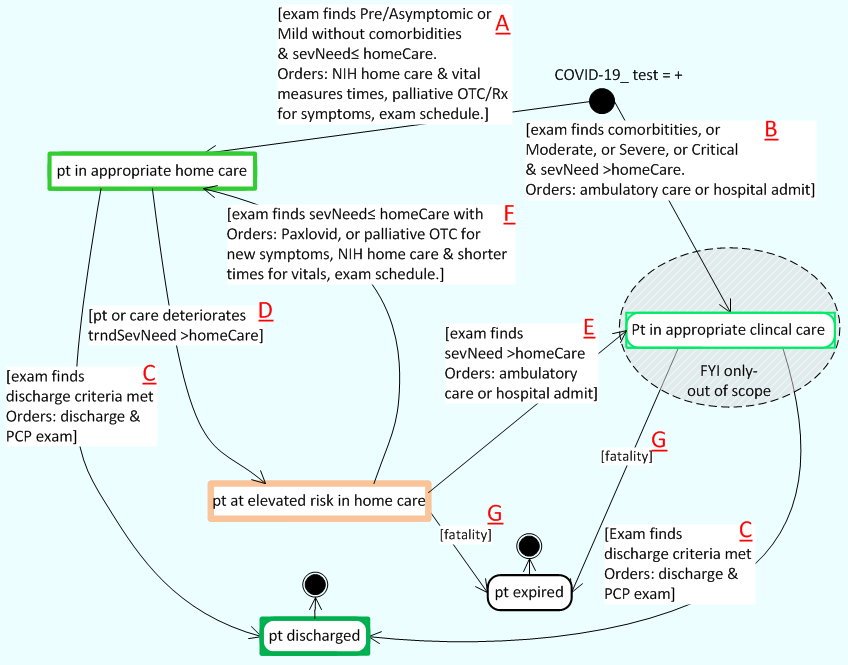
\includegraphics[width=3.35in, height=4in]{cwp.png}
    \end{tabular}
  \end{center}
\caption{The \href{https://github.com/ericmercer/SPIN-bpmn-cwp-verification-paper/blob/main/26-Oct-2021-CWP.png}{CWP} for remote COVID-19 patient care.}
\label{fig:cwp}
\end{figure}